\documentclass{beamer}
%
% Choose how your presentation looks.
%
% For more themes, color themes and font themes, see:
% http://deic.uab.es/~iblanes/beamer_gallery/index_by_theme.html
%
\mode<presentation>
{
	\usetheme{CambridgeUS}      % or try Darmstadt, Madrid, Warsaw, ...
	\usecolortheme{rose} % or try albatross, beaver, crane, ...
	\usefonttheme{structurebold}  % or try serif, structurebold, ...
	\setbeamertemplate{navigation symbols}{}
	\setbeamertemplate{caption}[numbered]
} 

\usepackage[english]{babel}
\usepackage[utf8]{inputenc}
\usepackage{multicol}
\usepackage{color}

\title[NCAA Basketball]{Data Analysis: Winning in NCAA Basketball}
\author{Justin Gomez \& Paul Harmon}

\date{April 27, 2017}

\begin{document}
	
	\begin{frame}
		\titlepage
	\end{frame}
	
	% Uncomment these lines for an automatically generated outline.
	%\begin{frame}{Outline}
	%  \tableofcontents
	%\end{frame}

	\section{Introduction}
	
	\begin{frame}{College Basketball}
	\begin{multicols}{2}
		\begin{itemize}
		\item College Basketball is a big deal! 
		\item CBS paid 10 billion dollars to broadcast the NCAA Men's tournament in 2015 
		\item Institutional credibility and culture 
		\item Student quality, retention
		\item Winning teams change campus cultures
				
		
	\end{itemize}
\textbf{Key Question}:\textit{What factors are associated with winning home games? }
	\begin{figure}[r]
		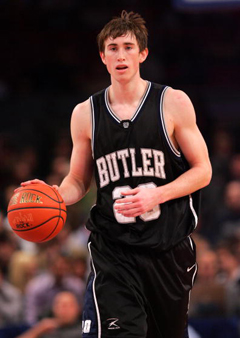
\includegraphics[height = .8\textheight]{hayward.jpg}
	\end{figure}
\end{multicols}
	
	\end{frame}

\begin{frame}{Research Questions}
\begin{enumerate}
	\item %1
	Which factors are most important in helping a home team win a game?
	\item %2
	Do the effects of each covariate on the probability of winning change in games that go to overtime?
	\item %3
	Can winning at home be accurately predicted?
\end{enumerate}
	
\end{frame}

	
\section{Data}
\begin{frame}{The Data}
	Data are obtained from Kaggle.com's repository for the 2016 March Machine Learning Mania competition. %Most of the people competing in this used predictive algorithms like random forests, etc. to predict outcomes; however, we used a logistic regression GLM. 
		\\
		\begin{itemize}
			\item 14 seasons, every college basketball game played
			\item More than 64,000 total games in the dataset  
						
		\end{itemize}
	
	\begin{figure}
		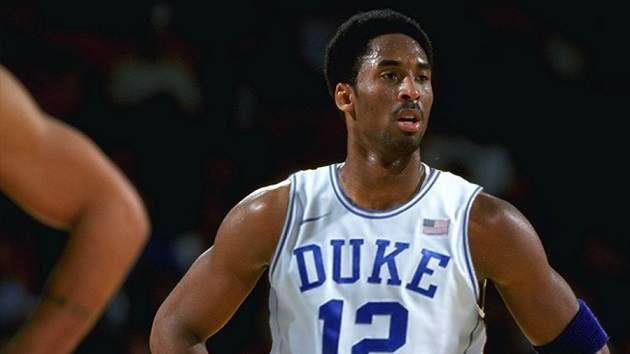
\includegraphics[width = 200 pt]{fakekobe.jpg}
	\end{figure}
	
\end{frame}

\begin{frame}{Variables}
\textbf{Response variable}: 1 if Home team won the game, 0 if the home team lost\\
Predictor variables are given as \textbf{differentials} (winning team stat - losing team stat) 

	\begin{multicols}{2}
		
	\begin{itemize}
		\item Field Goal Percentage
		\item Three Point Shooting Percentage
		\item Free Throw Shooting Percentage
		\item Turnovers
		\item Assists
		\item Steals
		\item Blocks
		\item Personal Fouls
		\item Total Rebounds
		\item Overtime (0 if not, 1 if yes)
	\end{itemize}
	
\end{multicols}


\end{frame}

\begin{frame}{Data Summaries}
	\centering
	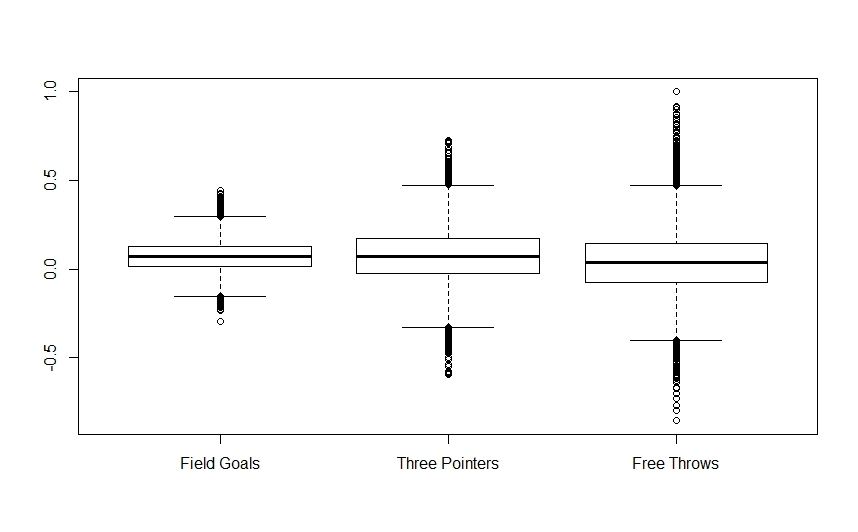
\includegraphics[height=.45\textheight]{percentbox.jpeg}\\
	\vspace{-15pt}
	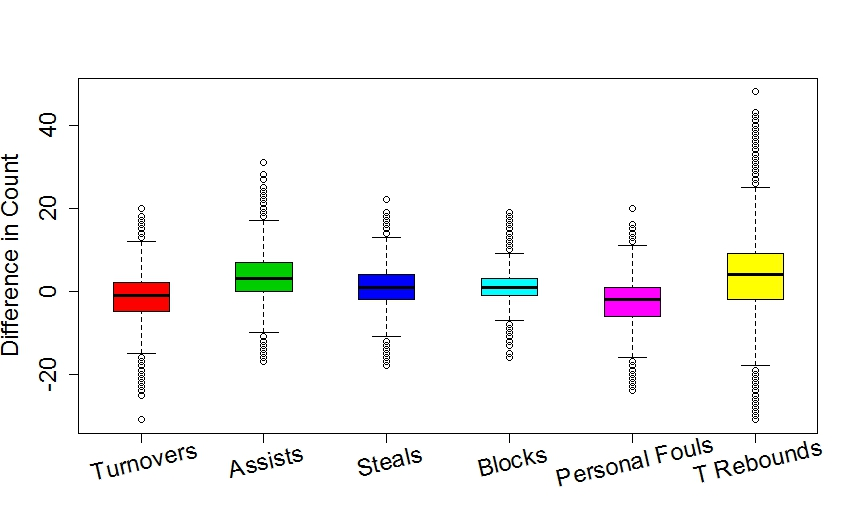
\includegraphics[height=.5\textheight]{diffbox.jpeg}
\end{frame}

\begin{frame}{Data Summaries}
	\centering
	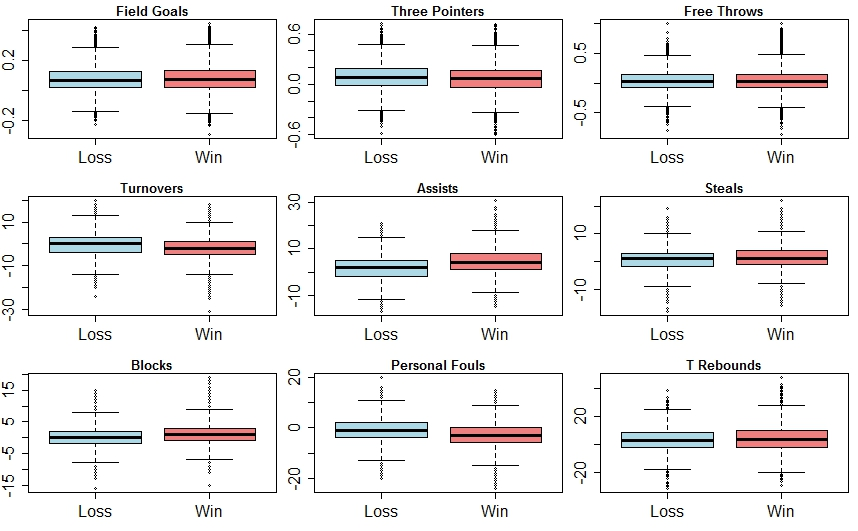
\includegraphics[height=.85\textheight]{toomanyboxes.jpeg}
\end{frame}

\begin{frame}{Prediction and Inference} 
Of secondary interest: how well does the GLM fitted to answer the first two research questions predict?
\begin{itemize}
	\item Training Split: 70\% of the data
	\item Testing Split: Remaining 30\%
	\item Misclassification rate will be found on testing set
\end{itemize}
\begin{figure}[r]
	
\includegraphics[height = .5\textheight]{fakelebron.png}
\end{figure}
\end{frame}

	
	\section{Methods}
	
	\begin{frame}[t]{Logistic Regression}
	Since the response is binary, we chose to fit a model with the \textbf{logit} link. We picked the logit link function for several reasons: 
	\begin{itemize}
		\item Logit - link allows for interpretation on probability scale
		\item Probit: It did not make sense to model game outcomes on a latent variable scale
		
	\end{itemize}
\textbf{Systematic Component}: 
\begin{eqnarray} \label{eq:logit}
\centering
logit(\pi_{i})=\beta_{0}+\sum_{j=1}^{p} \beta_{j}x_{ij}
\end{eqnarray} 
\textbf{Random Component}: 
\begin{equation}
\centering
Y_i \sim Bern(\pi_i)
\end{equation}
	\end{frame}
	

\begin{frame}{Model Space}
Three models were considered:
\begin{itemize}
	\item Full Interaction Model: All ten main effects, and pairwise interactions with overtime
	\item Reduced Interaction Model: All main effects with only pairwise interactions between ot and field goals, turnovers, and total rebounds
	\item Additive model: All ten main effects only
\end{itemize}
\begin{table}[h]
	\centering
	\begin{tabular}{rrr}
		\hline
		& AIC & Change in AIC \\ 
		\hline
		Reduced Interaction Model & 47803.16 & 0.00 \\ 
		Full Interaction Model & 47813.61 & 10.45 \\ 
		Additive Model & 47822.13 & 18.96 \\ 
		\hline
	\end{tabular}
\end{table}
\end{frame}	
	
\section{Results}

	\begin{frame}{The Model}
	The final theoretical model (reduced interaction model): 
	\begin{multline*}
	logit(\pi_{i})=\beta_{0}+\beta_{1}ot_{i}+\beta_{2}fgp_{i}+\beta_{3}tpp_{i}+\beta_{4}ftp_{i}+\beta_{5}todiff_{i}+\\
	\beta_{6}astdiff_{i}+\beta_{7}stldiff_{i}+\beta_{8}blkdiff_{i}+\beta_{9}pfdiff_{i}+\beta_{10}ot_{i}\times fgp_{i}\\
	+\beta_{11}ot_{i}\times todiff_{i}+\beta_{12}ot_{i}\times trdiff_{i}
	\end{multline*}
\begin{itemize}
	\item Hosmer-Lemeshow test gives large p-value (0.245), indicating a lack of evidence of poor fit
\end{itemize}	
\end{frame}	

\begin{frame}{The Estimated Model}
% latex table generated in R 3.3.2 by xtable 1.8-2 package
% Mon Apr 24 19:39:03 2017
\begin{table}[ht]
	\centering
	\begin{tabular}{rrrr}
		\hline
		& Lower Bound & Estimate & Upper Bound \\ 
		\hline
		Intercept & 0.78 & 0.81 & 0.84 \\ 
		Overtime & 0.99 & 1.10 & 1.23 \\ 
		Field Goal \% & 0.18 & 0.26 & 0.37 \\ 
		Three Point \% & 0.57 & 0.67 & 0.79 \\ 
		Free Throw \% & 1.37 & 1.56 & 1.78 \\ 
		Turnovers & 0.89 & 0.90 & 0.90 \\ 
		Assists & 1.13 & 1.14 & 1.15 \\ 
		Steals & 0.97 & 0.97 & 0.98 \\ 
		Blocks & 1.15 & 1.16 & 1.17 \\ 
		Personal Fouls & 0.86 & 0.87 & 0.87 \\ 
		Total Rebounds & 1.03 & 1.03 & 1.04 \\ 
		Overtime:Field Goal \% & 0.00 & 0.02 & 0.12 \\ 
		Overtime:Turnovers & 1.03 & 1.06 & 1.09 \\ 
		Overtime:Total Rebounds & 0.96 & 0.97 & 0.99 \\ 
		\hline
	\end{tabular}
\end{table}
\end{frame}	

\begin{frame}{Some Interpretations}
 
\begin{itemize}
	\item \textbf{Assists}: Holding other variables constant (including OT), in games where the winning team had one additional assist relative to the losing team's assists, the odds of the home team winning increased by between 13 and 15 percent. 
	\item \textbf{Turnovers}: In games that did not go to overtime, and holding other variables constant, in games where the winning team had an additional turnover relative to the losing team, the odds of the home team winning decreased by between 10 and 11 percent. If the game went to overtime, that decrease in the odds of the home team winning actually \textit{increased} relative to non-OT games by 3 to 9 percent. 
	

\end{itemize}
Most results lined up with what we expected. However, the estimate for Field Goal percentage was surprising. Possible issues multicollinearity could be an issue, or it may be that teams that shot fewer times also tended to have higher percentages even though they lost.  


\end{frame}
	
	
	
\begin{frame}{Answering Research Questions}
Recall our primary research questions: 

\textbf{Which factors are most important in helping a home team win a game?}
\begin{itemize}
	\item All variables are statistically significant, but this is expected given large sample size
	\item Practically important variables: \textcolor{red}{field goals}, \textcolor{red}{three points}, \textcolor{blue}{free throws}, \textcolor{blue}{assists}, \textcolor{blue}{blocks}
	\end{itemize}
		
\textbf{Do the effects of each covariate on the probability of winning change in games that go to overtime?}
\begin{itemize}
	\item The effects of Field Goal \%, Turnovers, and Total Rebounds appear to change in games that go to overtime
\end{itemize}



\end{frame}	

\begin{frame}{Checking Prediction}
A good inferential model should also be able to predict reasonably well (although not well enough to beat out Random Forest methods, etc.). We tested the model against our testing set and found a misclassification rate of 27.12\%. 
\begin{figure}
	\centering
	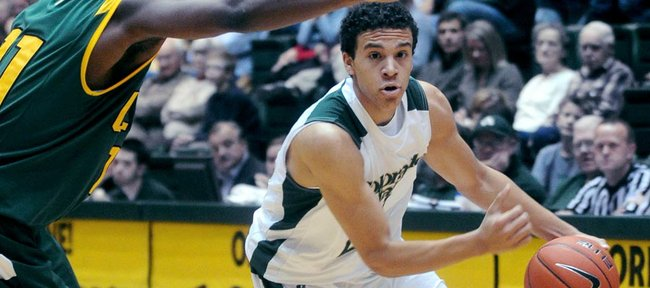
\includegraphics[height = 100pt]{dorian.jpg}
	\end{figure}
\end{frame}

\begin{frame}{Discussion}
\begin{itemize}
\item The response in this analysis considers specifically whether the home team won or lost
\item May be interesting to consider covariates that are not differentiated with home/away as an indicator variable (team level stats rather than game level)
\item So many games were considered in this analysis, tests for significance may not be as meaningful as we'd like them to be. 
\end{itemize}
\begin{figure}
	\centering
	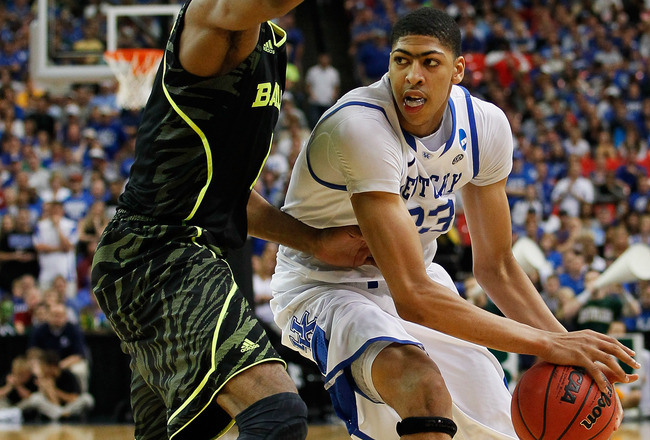
\includegraphics[height = 100pt]{unibrow.jpg}
\end{figure}
\end{frame}

\begin{frame}{References}
\begin{thebibliography}{4}
\bibitem{Advert}
Smith, D. Randall. (2008) Big Time College Basketball and the Advertising Effect: Does Success Really Matter? \textit{Journal of Sports Economics} Volume 9 No. 4 pp 387-406.
\bibitem{Econ}
Ogus, Simon. (2016) The Economic Impact of March Madness From First Four to Final Four. \textit{Forbes}. 

\bibitem{Agresti}
Agresti, A. (2015). \textit{Foundations of Linear and Generalized Linear Models}. Somerset: Wiley.
\end{thebibliography}
\centering

\includegraphics[height=100pt]{fakekobe2.jpg}

\end{frame}
	
\end{document}
